\section{The Thorin condition and what this book shows}\label{ch:intro}

Write $\xi(s)=\frac12s(s-1)\pi^{-s/2}\Gamma(s/2)\zeta(s)$ for the completed zeta function. It is entire of order one, real on the real axis and on the critical line, symmetric under $s\mapsto1-s$, and its zeros are the nontrivial zeros $\rho$ of $\zeta$. The Riemann Hypothesis (RH) asserts that every $\rho$ has real part $\frac12$.

This book works with a reformulation. Put
\[
G(u)=\frac{\xi(\frac12+\sqrt u)}{\xi(\frac12)} .
\]
Because $\xi(\frac12+s)$ is even in $s$, $G$ is an entire function of $u$ with no branch point, of order one half, and Hadamard's theorem gives
\[
G(u)=\prod_k\Big(1+\frac u{a_k}\Big),\qquad a_k=-(\rho_k-\tfrac12)^2,
\]
one factor for each pair $\{\rho,1-\rho\}$ (Section~\ref{ch:clock} derives the product as \eqref{eq:ch2:hadamard}). A zero on the line has $a_k=\gamma_k^2>0$; a zero off the line has $a_k$ complex. The reciprocal $1/G$ is the \emph{clock}. The classical theory of generalised gamma convolutions (GGC) of Thorin and Bondesson \cite{Thorin77a,Thorin,Bondesson} says that a function of the form $\exp\{-\int\log(1+u/z)\,U(dz)\}$ with a positive measure $U$ is the Laplace transform of a positive random variable, and that $U$, the Thorin measure, is unique. The rigidity theorem of \cite{P26}, which Section~\ref{ch:clock} restates with its source as Proposition~\ref{prop:rigid}, says that the clock $u\mapsto\xi(\frac12)/\xi(\frac12+\sqrt u)$ is the Laplace transform of a generalised gamma convolution if and only if RH holds, and that its Thorin measure is then
\begin{equation}\label{eq:URH}
U_{\RH}=\sum_{\gamma>0}\delta_{\gamma^2},
\end{equation}
while the clock variable is $T=\sum_{\gamma>0}e_\gamma/\gamma^2$ with independent standard exponentials $e_\gamma$.

We call the requirement that the Thorin measure of the clock be a positive measure the \emph{Thorin condition}. It has several equivalent faces, each of which is a sign condition. The logarithmic derivative $G'/G(u)=\sum_k(u+a_k)^{-1}$ must be a Stieltjes transform. The heat trace $W(t)=\sum_ke^{-a_kt}$ must be completely monotone. The Thorin density $\rho_\varepsilon(\theta)=\pi^{-1}\re(\xi'/\xi)(\frac12+\varepsilon+i\theta)$ at every resolution $\varepsilon>0$ must be nonnegative, which is Lagarias's criterion \cite{Lagarias}; for $\varepsilon\ge\frac12$, where the basepoint $\frac12+\varepsilon$ is at least one, it is positive with no hypothesis (Section~\ref{ch:basepoint}). Weil's explicit formula functional must be positive on positive definite test functions \cite{Weil52}. The clock must be hyperbolically completely monotone (Corollary~\ref{cor:hcm}). All of these say the same thing, and all of them are, at a finite resolution and on a finite window, computable. Section~\ref{sec:ch3:diag} turns them into tests and compares how well each locates a failure (Table~\ref{tab:ch3:diag}).

\subsection{What computation can and cannot say}

Computation has a long history in the study of RH. Riemann computed the first zeros by hand \cite{Siegel32}. Gram \cite{Gram03}, Backlund \cite{Backlund14}, Hutchinson \cite{Hutchinson25} and Titchmarsh \cite{Titchmarsh36} extended the tables \cite[Chapters 6 to 8]{Edwards}; Turing gave the method that certifies a count without evaluating off the line \cite{Turing53}; Lehmer found the near coincident pairs \cite{Lehmer56} that bound the de Bruijn Newman constant \cite{CSV94}; Odlyzko computed zeros near the $10^{12}$th zero, at height about $2.7\times10^{11}$, and tested their statistics against random matrix theory \cite{Odlyzko87}, and later computed zeros near the $10^{20}$th, at height about $1.5\times10^{19}$ \cite{Odlyzko92}, and beyond \cite{Odlyzko01}; Platt and Trudgian verified RH below height $3\times10^{12}$ \cite{PT21}. Appendix~\ref{app:history} tells this history, with the landmarks in Table~\ref{tab:appB}. None of it proves RH, and the reason is structural rather than technological: every computation sees finitely many zeros, and there are functions with the order, type and symmetry of $\xi$ that pass a given finite set of heat trace tests and yet have zeros off the line just above any sufficiently large height $R$ for which RH has been verified up to $R+50$ (Theorem~\ref{thm:ch13:perturb} \cite[Theorem D]{P17}).

The Thorin condition gives computation a different role. Instead of locating zeros one at a time, it asks for the sign of a measure, and the measure can be computed at every positive resolution without knowing where a single zero is. The questions then become quantitative. How close, in which metric, is the computed Thorin measure to the discrete RH measure? At what resolution does an off line zero become visible, and with what signature? What does the explicit formula say about the cost of computing the Thorin measure from the primes? Which limiting procedures preserve positivity and which do not? And since positivity is a theorem once the basepoint is moved from $\frac12$ to one, how much of it survives as the basepoint moves back across the critical strip? The book answers these questions, the last of them in Chapters~\ref{chap:basepoint} to \ref{chap:almost}.

Three ways of evaluating $\xi$ appear throughout. The first is P\'olya's integral, $\Xi(\theta)=\int\Phi(u)\cos(\theta u)\,du$, with the P\'olya kernel $\Phi$, a positive, doubly exponentially decaying function built from the Jacobi theta function. The integral is exact and needs no primes and no zeros, and since $\Phi$ is analytic in a strip the trapezoid rule applied to it is spectrally accurate; the cost is the cancellation $e^{-\pi\theta/4}$, which the tilted contour of Section~\ref{ch:polya} largely removes. The second is the Riemann Siegel formula and its fast multi point descendant, the Odlyzko Sch\"onhage algorithm \cite{OS88}, the tools of choice at large height. The third is the explicit formula, which evaluates the same objects from the primes and the gamma factor; the sine squared lemma is its Thorin form.

The principle that ties them together is that the Thorin measure at resolution $\varepsilon$ is the Poisson smoothing of the zeros, and simultaneously the sine squared image of the primes. The first description makes it computable from any evaluator of $\xi$ off the line. The second explains why the primes alone cannot compute it near the line. In Selberg's smoothed explicit formula the prime cutoff $x$ plays the part of the resolution: if no zero has real part greater than $\frac12$, the error at resolution $\varepsilon$ is of order $x^{-\varepsilon}/(\varepsilon^2\log x)$, so that $k$ correct digits need $x\approx10^{k/\varepsilon}$, with primes up to $x^2$ (Section~\ref{sec:ch10:selberg}). Figure~\ref{fig:ch1:flow} shows the first description at work: the Thorin measure at decreasing resolution, sharpening onto the zeros.

\begin{figure}[htbp]
\centering
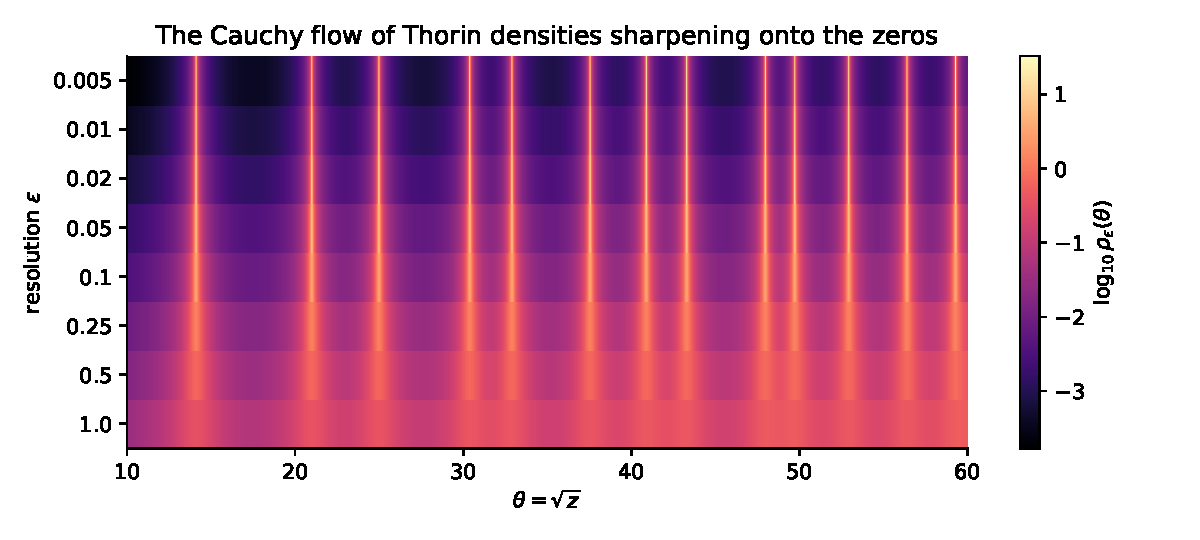
\includegraphics[width=\textwidth]{fig/flow.pdf}
\caption{The Thorin density $\rho_\varepsilon(\theta)$ on $10\le\theta\le60$, computed from the P\'olya density at eight resolutions from $\varepsilon=1$ (bottom) to $\varepsilon=0.005$ (top), on a logarithmic colour scale. As the resolution sharpens, the density concentrates on bright vertical lines at the ordinates of the zeros, all of which lie on the critical line in this window: the Cauchy flow converging to the RH measure $\sum\delta_{\gamma^2}$.}
\label{fig:ch1:flow}
\end{figure}

\subsection{Plan of the book and its principal results}

Two ideas set out in Sections~\ref{ch:clock} and \ref{ch:ggc} carry the rest of the book. The first, stated above, is that the Thorin measure at resolution $\varepsilon$ is the Poisson smoothing of the zeros and so is computable from any evaluator of $\xi$ off the critical line; as $\varepsilon\downarrow0$ it converges to the atoms on the line. The second is that the hierarchy of infinitely divisible laws becomes a hierarchy of positivity conditions on one function, the heat trace, of which the lower rungs are theorems and the top rung is RH. Every later chapter computes, tests or interprets one of these two ideas.

Chapter~\ref{chap:evaluation} evaluates $\xi$ and $\xi'$ in the complex plane by the P\'olya route, compares it with the classical evaluators and Turing's method, and follows one small computation from the theta series to a Thorin mass and a zero. Chapters~\ref{chap:measure} to \ref{chap:heat} are the core of the book. Chapter~\ref{chap:measure} measures the distance from the computed Thorin measure to $U_{\RH}$, computes the signature of an off line zero, reads the zero count and the zero density from the Thorin mass, and gives further readings of the sine squared lemma. Chapter~\ref{chap:hcm} treats weak convergence and hyperbolic complete monotonicity, brings in Bosch's theorem on powers of the half Cauchy law, and proves a theorem of the same shape for the clock, with a threshold set by the angle of the zeros. Chapter~\ref{chap:heat} climbs the hierarchy of positivity on the heat trace, explains what finite information cannot decide, computes the Thorin functional from the primes and relates the cell distance of Section~\ref{ch:distances} to the spacings of the zeros.

Chapters~\ref{chap:rzeta} and \ref{chap:rzid} study the reciprocal zeta function in the variable $u$ of the clock. The first gives its Thorin type forms and treats the gamma factor, the Meixner law and the sine squared lemma; the second proves that the normalised reciprocal zeta function is infinitely divisible and places it in the Bondesson hierarchy, then truncates the representation, due to Biane, Pitman and Yor, of $\xi$ as the Mellin transform of a GGC with Thorin atoms on a quadratic lattice and studies the conditions on the zeros of the truncations that would imply RH. Chapter~\ref{chap:probability}, with the P\'olya route as its evaluator, treats the clock as a random variable, through its law, its Kent approximants and its Brownian boundaries; it then turns to criteria other than the Thorin condition, the Keiper Li coefficients and the de Bruijn Newman flow, carries the evaluator to the $L$ functions of the character $\chi_{12}$, whose theta series is the Dedekind eta function, and of Ramanujan's $\Delta$, and recovers the zeros from the Thorin density by nonnegative deconvolution.

Chapters~\ref{chap:basepoint} to \ref{chap:almost} move the basepoint. The shifted clock $T_\alpha$ has Laplace transform $\xi(\alpha)/\xi(\alpha+\sqrt u)$; at $\alpha=\frac12$ it is the clock, and from $\alpha=1$ on its Thorin measure is positive with no hypothesis. These chapters carry both ideas from the basepoint one, the resolution $\varepsilon=\frac12$, into the critical strip. Chapter~\ref{chap:basepoint} works out the basepoint one, from the Mellin side, where $2\xi$ is a moment function of Bessel hitting times, to the Thorin measure and the law of $T_1$, and constructs $T_\alpha$ as a hitting time at every basepoint $\alpha>\frac12$. Chapter~\ref{chap:strip} extends the hierarchy to symmetric laws on the line, where the reciprocal of $\xi$ on the real axis is the characteristic function of a normal scale mixture, reads zero free half planes as completeness statements after Wiener, Salem and Riesz, and writes Riesz's criterion as the statement that every $T_\alpha$ with $\alpha>\frac12$ is a GGC. Chapter~\ref{chap:almost} reads the hierarchy through the books of Sato and Bondesson, repeats the calculations at the basepoint one for $L(s,\chi_{12})$, uses zero density estimates to bound how far each $T_\alpha$ can be from a GGC, and closes with the work of Anthony Pakes on size biasing, the Lambert law and ladders of self decomposable laws.

Chapter~\ref{chap:conclusions} assembles the results of the preceding chapters into a path towards RH on which every step is marked proved, computed, announced or open, sets out the computations that remain as one programme with its milestones, and draws the lessons of the computations for the Thorin programme. Chapter~\ref{chap:ferro} reads RH as a statement about one law, that the P\'olya variable is ferromagnetic, in the sense that its moment generating function vanishes only on the imaginary axis; it develops the class of such laws, checks the necessary conditions on the P\'olya law, builds, with no hypothesis, provably ferromagnetic laws within total variation distance $1.3\times10^{-4}$ of it and, by a computer assisted proof, within $2\times10^{-6}$, and shows that $e^{2X}$, a size biased form of the variable of Biane, Pitman and Yor, is self decomposable but not a generalised gamma convolution. Chapter~\ref{chap:maxwald} reads the P\'olya density as the density of a maximum order statistic of independent exponential variables and follows the clock through that representation: its Wald couple with the P\'olya variable, a criterion for the Thorin condition, an explicit generalised gamma convolution within a certified Laplace distance of it, the finite stages of the maximum and the Bondesson classes. Chapter~\ref{chap:phase} places the computations of the book on the Thorin phase diagram of the de Bruijn Newman flow, the set of points $(t,\alpha)$ at which the shifted clock of $\xi_t$ is a generalised gamma convolution, over which the minimum of $t+2(\alpha-\frac12)^2$ is the de Bruijn Newman constant, and certifies the finite part of one of its points below height $160$. Appendix~\ref{app:code} describes the code, the scripts and the data files behind the tables and figures, Appendix~\ref{app:history} gives a short history of computations on the zeros, Appendix~\ref{app:notation} lists the notation, and Appendix~\ref{app:bosch} gives the verification code for the Bosch type theorem.

Tables~\ref{tab:intro:summary}, \ref{tab:intro:summary45} and \ref{tab:intro:summary6} collect the principal results of Chapters~\ref{chap:evaluation} to \ref{chap:almost}, each with the section where it is developed. A result is marked proved when that section proves it or cites a proof, and computed when it rests on a computation; the section states how far the computation is certified.

{\footnotesize
\begin{longtable}{p{0.60\textwidth}p{0.12\textwidth}p{0.17\textwidth}}
\toprule
Result & Status & Where\\
\midrule
\endfirsthead
\toprule
Result & Status & Where\\
\midrule
\endhead
\bottomrule
\endfoot
\bottomrule
\caption{Principal results of Chapters~\ref{chap:evaluation} to \ref{chap:heat}.}\label{tab:intro:summary}\\
\endlastfoot
P\'olya route: $\xi$ and $\xi'$ from two fixed polynomials in ball arithmetic, about $60$ correct digits at height $200$ at $420$ bits, $0.7$ ms per point & \raggedright computed & Section~\ref{ch:polya}\\
Tilted contour: $25$ digits of $\rho_{0.05}$ at height $5000$ against \texttt{mpmath}, in $28$ ms per point; to leading exponential order the loss to cancellation falls from about $0.341\,\theta$ digits to about $\delta\theta/\log10$ & \raggedright proved and computed & Section~\ref{ch:polya}\\
The Lehmer pair near height $7005$ resolved by the tilted P\'olya route at $34$ ms per point & \raggedright computed & Section~\ref{sec:ch5:lehmer}\\
$N(1000)=649$ from the Thorin mass at resolution $\frac12$ and the argument along a horizontal segment & \raggedright computed & Section~\ref{sec:ch5:count}\\
Raw total variation to $U_{\RH}$ maximal; matched total variation at the floor $3.7\times10^{-9}\varepsilon$ of the tail model; cell distance $5.44\,\varepsilon$ & \raggedright computed & Section~\ref{ch:distances}\\
Mass defect $-(\varepsilon/\pi)\Xi'(\Theta)/\Xi(\Theta)$ to first order; at $\Theta=200$ the observed slope agrees with it to five digits at $\varepsilon=0.005$ & \raggedright proved and computed & Section~\ref{ch:distances}\\
Signatures of an off line pair in total variation and negative mass, exact for an omitted pair and for the negative mass, to leading order for a displaced pair & \raggedright proved & Section~\ref{ch:offline}\\
Zero density $\nu(\frac12+\varepsilon,200)=0$ at eight resolutions, from the argument principle identity of Proposition~\ref{prop:zerodensity} & \raggedright computed & Section~\ref{ch:turing}\\
Prime side of the sine squared lemma: when no zero has real part greater than $\frac12$, Selberg's smoothed sum computes $\rho_\varepsilon$ with relative error at most $(x^{-\varepsilon}+x^{-2\varepsilon})/(\varepsilon\log x)$, so with error of order $x^{-\varepsilon}/(\varepsilon^2\log x)$ at the peaks, the single zero law; tested at $\varepsilon=\frac14$ & \raggedright proved and computed & Section~\ref{ch:sin2more}\\
The Thorin measures converge vaguely to the measure of the zeros on the line, whether or not RH holds & \raggedright proved & Section~\ref{ch:weak}\\
The clock is HCM if and only if RH holds, and the shifted clock at any basepoint $\alpha\ge1$ is HCM unconditionally; the $216$ normalised derivatives of a finite HCM test are all positive, certified in ball arithmetic & \raggedright proved and computed & Section~\ref{ch:weak}\\
Bosch type threshold: $1/G(x^{1/\beta})$ is HCM if and only if $|\beta|\ge1/(1-\alpha_\xi)$, with $\alpha_\xi$ set by the largest angle of the zeros; unconditionally $1/G(x^p)$ is HCM for $|p|\le1-1/(\pi T_0)$, where $T_0=3\times10^{12}$ is the verified height, in particular for $|p|\le1-1.1\times10^{-13}$ & \raggedright proved & Section~\ref{ch:boschB}\\
The clock is infinitely divisible and self decomposable with no hypothesis, and $(-1)^kW^{(k)}>0$ for every $k\le1.16\times10^{25}$, that is, the Williamson measures, inverse gamma smoothings of the Thorin measure, are positive to that order; the two proofs use the verification of RH below heights $1000$ and $3\times10^{12}$ respectively \cite{PT21}; Laplace's method on the Gumbel tail of the P\'olya kernel and a Tauberian argument give the leading term of the Weyl law & \raggedright proved & Section~\ref{ch:heat}\\
\end{longtable}}

{\footnotesize
\begin{longtable}{p{0.60\textwidth}p{0.12\textwidth}p{0.17\textwidth}}
\toprule
Result & Status & Where\\
\midrule
\endfirsthead
\toprule
Result & Status & Where\\
\midrule
\endhead
\bottomrule
\endfoot
\bottomrule
\caption{Principal results of Chapters~\ref{chap:rzeta} to \ref{chap:probability}.}\label{tab:intro:summary45}\\
\endlastfoot
The normalised reciprocal zeta function is infinitely divisible with no hypothesis, and it is not self decomposable, not a GGC and not in the Bondesson class & \raggedright proved and computed & Section~\ref{ch:rz3}\\
Conjecture S, that the symmetrised truncations of the Biane, Pitman and Yor lattice have their zeros in the strip on the line, holds for the sizes $n\le24$ and $n=32,36$ above explicit heights and numerically below them; for infinitely many $n$ it would imply RH & \raggedright proved and computed & Section~\ref{ch:rz4}\\
Law of the clock by Talbot inversion, with no zero as input; its hazard tends to $\gamma_1^2$, reached to eleven digits at $t=0.25$ & \raggedright computed & Section~\ref{ch:clocklaw}\\
Kent approximants with $1700$ zeros and a moment matched Weyl tail: relative error $3.5\times10^{-23}$ at $u=1$ and $7.0\times10^{-13}$ at $u=10^4$; for large $u$ the error of the plain Weyl tail levels off at a constant set by $S$ & \raggedright computed & Section~\ref{ch:clocklaw}\\
The clock is not the first passage time of Brownian motion to an independent random level; the boundary from the Volterra equation, solved in three zones, reproduces its law to Monte Carlo accuracy (Kolmogorov distance $0.0020$, against $0.0059$ for the tangent boundary) & \raggedright proved and computed & Section~\ref{ch:boundaries}\\
Keiper Li coefficients $\lambda_1,\dots,\lambda_{100}$ from the P\'olya density, $\lambda_1$ to $25$ digits & \raggedright computed & Section~\ref{ch:li}\\
Closest pair below height $200$ collides at de Bruijn Newman time $-0.288$; the Lehmer pair near $7005$ at $-7.11\times10^{-4}$ & \raggedright computed & Section~\ref{ch:dbn}\\
For $L(s,\chi_{12})$ and $L(s,\Delta)$ the sine squared lemma has no pole piece but a signed prime piece & \raggedright proved & Section~\ref{ch:chi12}\\
The eta kernel of $L(s,\chi_{12})$: GRH below height $100$ from the zero density identity and the $67$ sign changes & \raggedright computed & Section~\ref{ch:chi12}\\
For an imaginary quadratic field the P\'olya kernel of $\zeta_K$ is positive exactly when an explicit theta sum is positive on a finite interval, which gives $L(\frac12,\chi_d)>0$ for $d=-3,-4,-7,-8$; it takes negative values for every $d\equiv5\pmod{24}$ & \raggedright proved & Section~\ref{ch:chi12}\\
For the Dirichlet beta function $L(s,\chi_4)$, whose kernel is the cube of the eta function: GRH below height $100$; a positive Thorin density at every basepoint $\alpha\ge1$, which the absolute values of the prime weights certify only for $\alpha>2.2823$; the density as the difference of those of $\xi_{\mathbb Q(i)}$ and $\xi$, and as the derivative of the argument of the completed function on the line & \raggedright proved and computed & Section~\ref{sec:dbeta:beta}\\
Nonnegative deconvolution of $\rho_{0.1}$ on $[15,55]$, with the zeros outside $[5,65]$ as background, recovers every zero in the window to within $10^{-5}$ & \raggedright computed & Section~\ref{ch:deconv}\\
For P\'olya's Bessel function $K_{i\theta/2}(2\pi)$ the index side clock is the hitting time of an explicit diffusion, its Thorin atoms are the squared zeros and its trace is completely monotone; its de Bruijn Newman constant is finite, by Newman's theorem, although none of its real zeros below height $90$ collide down to $t=-60$ & \raggedright proved and computed & Section~\ref{ch:biane}\\
\end{longtable}}

{\footnotesize
\begin{longtable}{p{0.60\textwidth}p{0.12\textwidth}p{0.17\textwidth}}
\toprule
Result & Status & Where\\
\midrule
\endfirsthead
\toprule
Result & Status & Where\\
\midrule
\endhead
\bottomrule
\endfoot
\bottomrule
\caption{Principal results of Chapters~\ref{chap:basepoint} to \ref{chap:almost}. All are unconditional, and several use verified computations: the verification of RH below height $1000$, through Theorem~\ref{thm:ch12:idsd}, or below the height $T_0=3\times10^{12}$, Platt's verification of GRH for small moduli, or computations in ball arithmetic.}\label{tab:intro:summary6}\\
\endlastfoot
$T_1$, with Laplace transform $\xi(1)/\xi(1+\sqrt u)$, is a GGC with positive Thorin density, smallest at the origin, by a computation of the zeros below height $2000$ in ball arithmetic and explicit zero counts above it, so that $T_1$ is a positive stable one half variable plus an independent GGC; its law has infinite mean and a stable one half tail, and the L\'evy form of $\xi(1+s)$, which converges by the prime number theorem, gives its Thorin density from the primes & \raggedright proved and computed & Section~\ref{ch:basepoint}\\
Below the basepoint one, $v_\alpha(\theta)/(\alpha-\frac12)$ is nonincreasing in $\alpha$ away from the zeros off the line; the Thorin density is smallest at the origin, and only there, for every $\alpha\in(\frac12,7.35]$ on $|\theta|\le3\times10^{12}-1.21$, for $L(s,\chi_4)$ and $L(s,\chi_{12})$ at every height for every $\alpha\ge1$, and at every height for every $\alpha\in(\frac12,1)$ exactly when RH holds; for every $\alpha>\frac12$ it is positive on $|\theta|\le3\times10^{12}-\frac12$ & \raggedright proved and computed & Sections~\ref{sec:dbeta:comp}, \ref{ch:almost}\\
Every $T_\alpha$, $\alpha>\frac12$, exists as the tilted centre clock run through the inverse local time of a sticky Brownian motion, and it is a GGC if and only if no zero has real part greater than $\alpha$ & \raggedright proved & Section~\ref{ch:bphit}\\
For real $u$ and $\alpha\ge\frac12$, $\xi(\alpha)/\xi(\alpha+|u|)$ is the characteristic function of an infinitely divisible normal scale mixture; for $\frac12<\alpha<1$ it is an extended GGC, and the translates of every tilted P\'olya kernel $\Phi_{\alpha'}$ with $\alpha'>\alpha$ are complete in $L^1$, exactly when no zero has real part greater than $\alpha$ & \raggedright proved & Section~\ref{ch:strip}\\
The complete monotonicity conditions of the Poisson trace $K_{1/2}$, which together are RH, hold for every order $n<T_0(\pi-y)$ at the point $y$; $K_{1/2}$ and the trace of P\'olya's Bessel function differ by $\frac98+O(y\log\frac1y)$ as $y\to0$ & \raggedright proved and computed & Section~\ref{sec:biane:cm}\\
$1/\zeta(2k)$ is, up to an elementary factor, a value of the Laplace transform of the centre clock and of $T_1$; for $\frac12\le\alpha<1$ the bound $O(x^{\alpha/2+\delta})$ on Riesz's function, for every $\delta>0$, holds exactly when every $T_{\alpha'}$ with $\alpha'>\alpha$ is a GGC & \raggedright proved & Section~\ref{ch:riesz}\\
The constant of $\sum_{n\le x}\mu(n)^2/n$ is an elementary term plus $\E V_1-2\,\E V_2$, two tilted P\'olya means; RH holds exactly when the squarefree count smoothed by an exponential or a Gamma(2) law, or the count in mean square, has error $O(x^{1/4+\varepsilon})$; the error is $\Omega_\pm(x^{1/4})$; Gamma(2) smoothing writes it as an average of the Mertens function under a positive law, and two is the largest shape for which this holds & \raggedright proved & Section~\ref{sec:sqfree}\\
The centre clock is driven by a subordinator with L\'evy density $-W'$ and is unimodal, as is $T_\alpha$ for $\alpha\ge1$; the tilted P\'olya variable is quasi infinitely divisible for every $\alpha>1$ but not at $\alpha=1$ & \raggedright proved & Section~\ref{ch:sato}\\
For $L(s,\chi_{12})$ the Thorin measure at the basepoint one is positive, and its L\'evy form there has no pole to compensate and prime atoms of both signs & \raggedright proved & Section~\ref{ch:bpeta}\\
For $\frac12<\alpha<1$, in the density $\rho_{\alpha-1/2}$ the Cauchy kernels of the zeros to the right of $\alpha$ carry at heights $\theta\le T$ at most $T^{e(\alpha)-1+o(1)}$ times the mass of the kernels of the other zeros, with $e(\alpha)<1$, by the zero density estimates of Ingham, of Guth and Maynard and of Huxley \cite{Ingham40,GM26,Huxley72} & \raggedright proved & Section~\ref{ch:almost}\\
With no hypothesis, the size biased centre clock is the clock plus an independent variable with density $W/\E T$, and RH holds exactly when this variable is a mixture of exponential laws, with weight $\gamma^{-2}/\E T$ at the rate $\gamma^2$, about a fifth at the lowest zero; the Lambert law, with Laplace transform $\mathcal W(u)/u$, is a GGC whose Thorin measure is the image of the uniform law on $(0,\pi)$ under $b\mapsto b\,e^{-b\cot b}/\sin b$, by a proof of which only one step fails for the clock, and that step is RH & \raggedright proved and computed & Sections~\ref{pk:sec:form}, \ref{pk:sec:lambert}\\
The centre clock lies in Urbanik's class $L_2$ of multiply self decomposable laws and not in $L_3$; it is not the martingale limit of a supercritical continuous state branching process with finite Malthusian parameter & \raggedright proved and computed & Section~\ref{pk:sec:ladder}\\
A property of even kernels that also holds for the damped P\'olya kernel $e^{tv^2/4}\Phi(v)$ for some $t<0$ cannot by itself imply RH, by the theorem of Rodgers and Tao; the GGC property of the variable of Biane, Pitman and Yor fails for the damped kernel at every $t<0$ tested and, provably, for small $|t|$, so the filter does not exclude it there & \raggedright proved and computed & Section~\ref{pk:sec:filter}\\
\end{longtable}}

\subsection{Conventions and how to read this book}

The clock is a function of $u=s^2$, so that the atoms of its Thorin measure are at $\gamma^2$; earlier papers of the programme used $s^2/2$, which rescales Thorin measures by $z\mapsto z/2$. Thorin measures are measures in the variable $z$, and we write $\theta=\sqrt z$ for the chart in which the Thorin measure at the basepoint $\frac12+\varepsilon$ has density $\rho_\varepsilon(\theta)=\pi^{-1}\re(\xi'/\xi)(\frac12+\varepsilon+i\theta)$; $\varepsilon$ is the resolution. The P\'olya kernel $\Phi$ is taken in Titchmarsh's normalisation, $\Xi(\theta)=\int_{\mathbb R}\Phi(u)\cos(\theta u)\,du$. $N(T)$ counts zeros with $0<\im\rho\le T$ and $\nu(\sigma,T)$ those with, in addition, $\re\rho>\sigma$. Total variation of a signed measure is the total variation norm $|\mu|(E)$ on the stated window. Chapters~\ref{chap:rzeta} and \ref{chap:rzid}, and Sections~\ref{ch:boschA} and \ref{ch:boschB}, write $s$ for $u$, and the Kent approximants of Section~\ref{ch:clocklaw} write $w$; each declares its variables where it starts, and Appendix~\ref{app:notation} lists the notation of the book with the place where each symbol is defined. Numerical values are quoted to the accuracy at which they have been checked, and the section in which a value is computed says how.

Readers mainly interested in computation can read Sections~\ref{ch:clock}, \ref{ch:polya} and \ref{ch:worked} and then go straight to Chapters~\ref{chap:measure} to \ref{chap:heat}, where the Thorin condition is analysed numerically. Readers interested in the probabilistic side can start with Sections~\ref{ch:ggc}, \ref{ch:clocklaw} and \ref{ch:boundaries} and continue with Chapters~\ref{chap:basepoint} to \ref{chap:almost}, where the shifted clocks are hitting times and normal scale mixtures; these chapters build on Sections~\ref{ch:clock} and \ref{ch:ggc} and draw on Section~\ref{ch:turing} for the zero count. Chapters~\ref{chap:rzeta} and \ref{chap:rzid} can be read after Chapter~\ref{chap:foundations} and the statements of Theorems~\ref{thm:ch12:idsd} and \ref{thm:ch12:cm} in Section~\ref{ch:heat}; they form the most technical part of the book, and they prove unconditional theorems about the reciprocal zeta function. Readers looking for the conclusions can go directly to Sections~\ref{ch:path} and \ref{ch:lessons}. Throughout, statements are marked as proved, computed, announced or open, and Appendix~\ref{app:code} names the script behind each computed table and figure or records that the archive has none.
